\section{Signature for Sequential Circuit}
In this section, I discussed the signature for two sequential circuits, i.e., 3-bit counter and FIR filter.
\subsection{3-bit Counter}

Figure~\ref{fig:matlab} shows the 3-bit counter in MATALB Simulink. I have derived the signature by stuck-at-fault model to all different possible nodes. Table~\ref{stuck}  shows the signature if the node B0 stuck at "1." Similarly, I have derived the signatures of all other nodes\footnote{due to space constraints I didn't provide all the signatures}.

\begin{figure}[tb!]
 \centering
  \captionsetup{justification=centering}    
   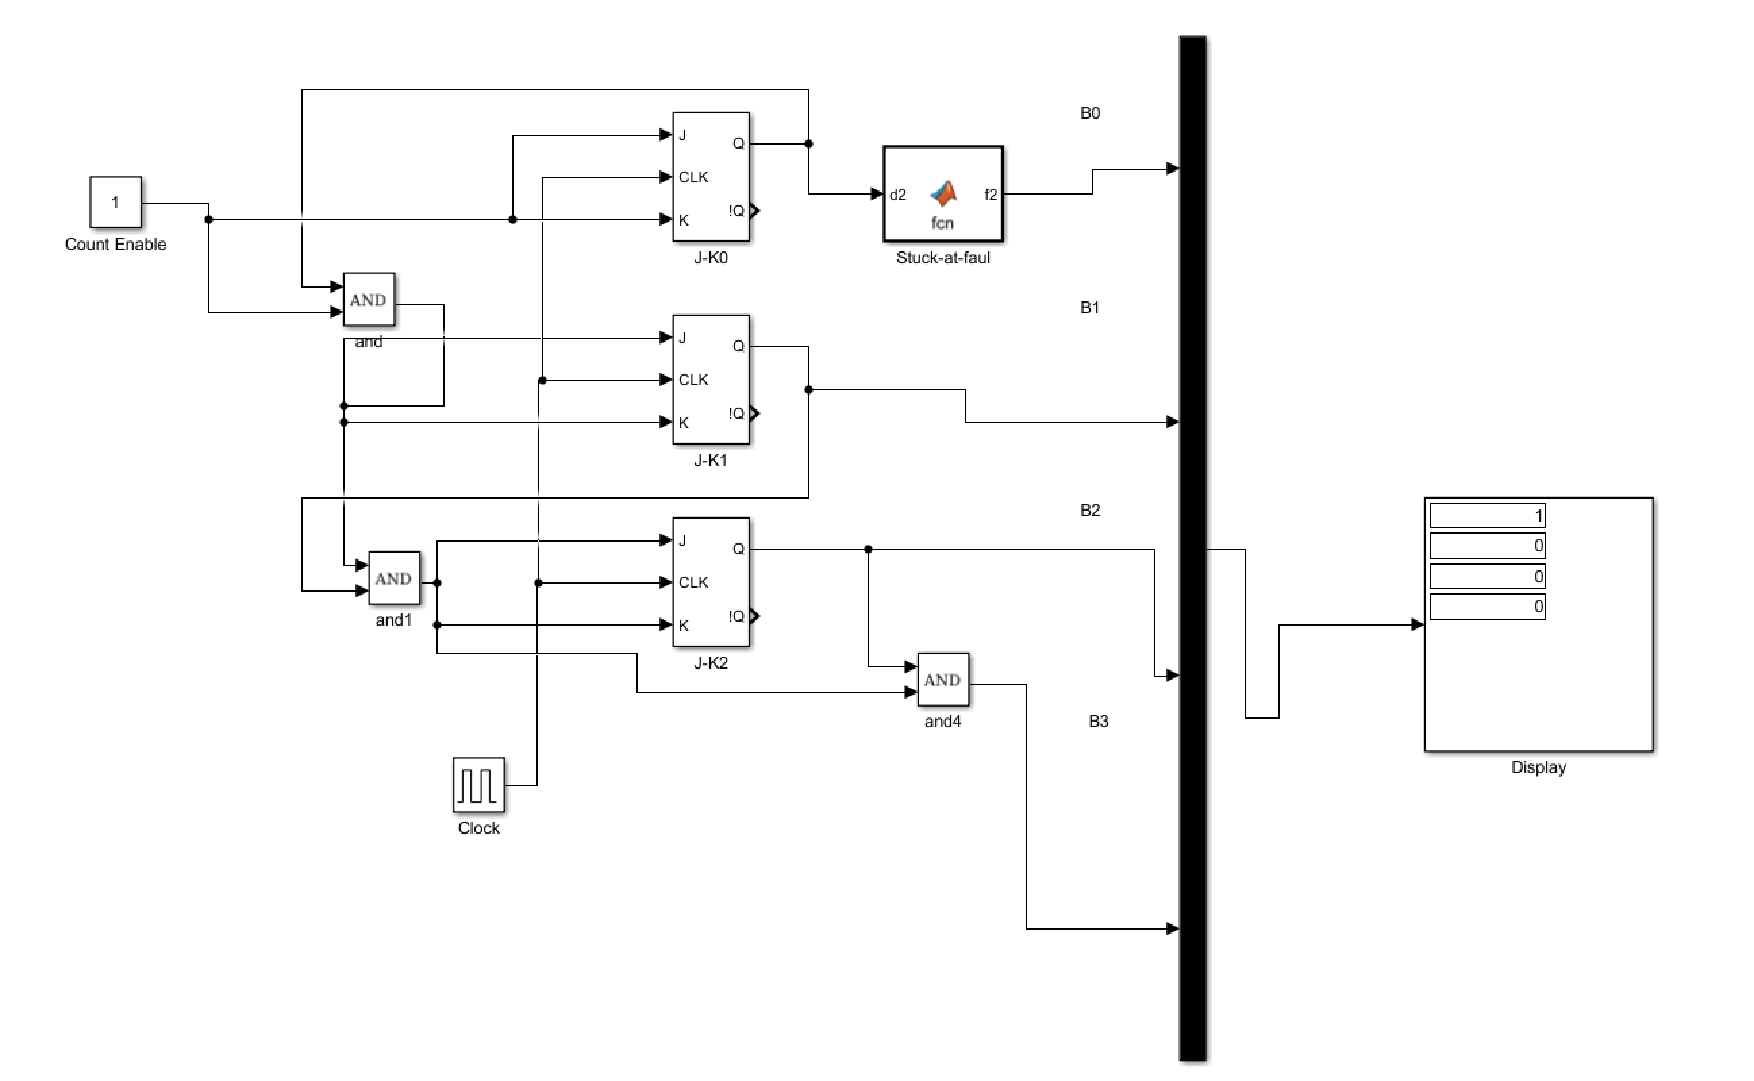
\includegraphics[scale=0.6]{Figures/matlab-counter.pdf}
   \caption{3-bit counter in MATALB.}
\label{fig:matlab}
\end{figure}

\begin{table}[tb!]
\center
\caption{Stuck-at-1$\rightarrow B_0$.}
\label{stuck}
\begin{tabular}{|c | c| c | c| } 
 \hline
 \rowcolor{lightgray}
Faulty Value (Binary) & Faulty Value & Original Value & Arithmetic Signature   \\ 
\hline
 
 
 001& 1 &0 & -1  \\
 \hline
 011 & 3 & 1 & -2 \\ 
 \hline
 
 101 & 5 & 2 & -3 \\
 \hline
 111& 7& 3& -4 \\
 \hline
 001 & 1  &  4& 3 \\
 \hline
 011 & 3 & 5 &2  \\
 \hline
 101 & 5 & 6 & 1 \\
 \hline
 111 & 7 & 7 & 0 \\
 \hline
 
 
\end{tabular}
\end{table}

\subsection{Signature for FIR Filter}


In this example, I have applied stuck-at-fault model to different nodes in the FIR filter as shown in Figure~\ref{fig:filter} and find their respective Signatures as shown in Table~\ref{firtable1}, Table~\ref{firtable2}.
%
%\textbf{MATLAB code}
%
%\begin{lstlisting}[frame=single]  % Start your code-block
%
%
%
%xn = [0 1 2 3 4 5 6 7 6 5 4 3 2 1];
%xn_1 = [0 0 1 2 3 4 5 6 7 6 5 4 3 2 1 0];
%
%A = [0 1 2 3 2 3 1 0 0 1 2 3 2 3 1];
%
%B = [0 1 2 3 2 3 1 0 0 1 2 3 2 3 1];
%
%y = xn .* A + xn_1 .* B
%
%
%\end{lstlisting}



\begin{figure}[tb!]
 \centering
  \captionsetup{justification=centering}    
   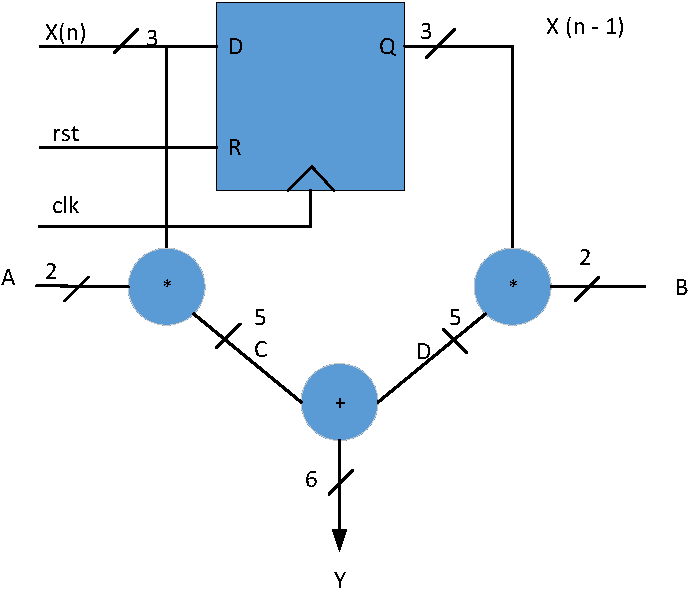
\includegraphics[scale=0.6]{Figures/FIR.pdf}
   \caption{FIR Filter.}
\label{fig:filter}
\end{figure}





\begin{table}[tb!]
\center
\caption{Stuck-at-0$\rightarrow Y_0$}
\label{firtable1}
\begin{tabular}{|c | c| c | c| c |} 
 \hline
 \rowcolor{lightgray}
Decimal Golden & Binary & Stuck@0$\rightarrow Y_0$ & Decimal Faulty & Arithmetic Signature   \\ 
\hline
 
 
 0 & 000000 & 000000 & 0 & 0  \\
 \hline

 1 & 000001 & 000000 & 0 & 1 \\
 \hline
 
 6 & 000110 & 000110 & 6 & 0 \\
 \hline
 15 & 001111 & 001110 & 14 & 1 \\
 \hline
 14 & 001110 & 001110 & 14 & 0 \\
 \hline
 27 & 011011 & 011010 & 26 & 1 \\
 \hline
 11 & 001011 & 001010 & 10 & 1 \\
 \hline
 0 & 000000 & 000000 & 0 & 0 \\
 \hline
 0 & 000000 & 000000 & 0 & 0 \\
 \hline
 11 & 001011 & 001010 & 10 & 1 \\
 \hline
 18 & 010010 & 010010 & 18 & 0 \\
 \hline
 
 21 & 010101 & 010100 & 20 & 1 \\
 \hline
 10 & 001010 & 001010 & 10 & 0 \\
 \hline
 9 & 001001& 001000 & 8 & 1 \\
 \hline
 1 & 000001 & 000000 & 0 & 1 \\
 \hline
 0 & 000000 & 000000 & 0 & 0 \\
 \hline




 
 
\end{tabular}
\end{table}






\begin{table}[tb!]
\center
\caption{Stuck-at-1$\rightarrow C_3$}
\label{firtable2}
\begin{tabular}{|c |c | c | c| c | c| c |} 
 \hline
 \rowcolor{lightgray}
Decimal Golden & C & C-Binary & Stuck@1$\rightarrow C_3$ & Decimal & Faulty &Signature   \\ 
\hline
 
 
 0 & 0 & 00000 & 01000 & 8 & 8 &-8  \\
 \hline

 
  1 & 1 & 00001 & 01001 & 9 & 9 &-8  \\
 \hline
  
   6 & 4 & 00100 & 01100 & 12 & 14 &-8  \\
 \hline


 
  15 & 9 & 01001 & 01001 & 9 &  15 & 0 \\
 \hline
  
    14 & 8 & 01000 & 01000 & 8 &  14 & 0 \\
 \hline

  27 & 15 & 01111& 01111 & 15 &  27 & 0 \\
 \hline
 
  11 & 6 & 00110 & 01110 & 14 &  19 & -8 \\
 \hline
 
  0 & 0 & 00000 & 01000 & 8 &  8 & -8 \\
 \hline
 
  0 & 0 & 00000 & 01000 & 8 &  8 & -8 \\
 \hline
   
  11 & 5 & 00101 & 01101 & 13 &  19 & -8 \\
 \hline
 
  18 & 8 & 01000 & 01000 & 8 &  18 & 0 \\
 \hline
  21 & 9 & 01001 & 01001 & 9 &  21 & 0 \\
 \hline
  10 & 4 & 00100 & 01100 & 12 &  18 & -8 \\
 \hline
  9 & 3 & 00011 & 01011 & 11 &  17 & -8 \\
 \hline
 
  1 & 0 & 00000 & 01000 & 8 &  9 & -8 \\
 \hline
 
  0 & 0 & 00000 & 01000 & 8 &  8 & -8 \\
 \hline
 
 
 
 
 
 
 
 
 
 
 
 
 
 
 
 
 
\end{tabular}
\end{table}













